\documentclass[12pt,a4paper,t,xcolor=dvipsnames,slidestop,compress,mathserif]{beamer}
\usepackage{amsmath,amssymb,graphicx,color,multicol,amsfonts,algorithmic,url,stmaryrd,epsf}
\usepackage{graphicx, algorithm2e}

%% ----------------------------------------------------------------------
%% Definitions, Macros, Etc.
%% ----------------------------------------------------------------------

%% Hyper-linked References
\newcommand{\Sec}[1]{\hyperref[sec:#1]{\S\ref*{sec:#1}}} %section
\newcommand{\Eqn}[1]{\hyperref[eq:#1]{(\ref*{eq:#1})}} %equation
\newcommand{\Fig}[1]{\hyperref[fig:#1]{Figure~\ref*{fig:#1}}} %figure
\newcommand{\Tab}[1]{\hyperref[tab:#1]{Table~\ref*{tab:#1}}} %table
\newcommand{\Thm}[1]{\hyperref[thm:#1]{Theorem~\ref*{thm:#1}}} %theorem
\newcommand{\Lem}[1]{\hyperref[lem:#1]{Lemma~\ref*{lem:#1}}} %lemma
\newcommand{\Prop}[1]{\hyperref[prop:#1]{Property~\ref*{prop:#1}}} %property
\newcommand{\Cor}[1]{\hyperref[cor:#1]{Corollary~\ref*{cor:#1}}} %corollary
\newcommand{\Def}[1]{\hyperref[def:#1]{Definition~\ref*{def:#1}}} %definition
\newcommand{\Alg}[1]{\hyperref[alg:#1]{Algorithm~\ref*{alg:#1}}} %algorithm
\newcommand{\Ex}[1]{\hyperref[ex:#1]{Example~\ref*{ex:#1}}} %example

% Theorem-like constructs
%\newtheorem{example}[theorem]{Example}

% Blackboard fonts 
\newcommand{\Real}{\mathbb{R}}
\newcommand{\Cplx}{\mathbb{C}}
%% Transposes
\newcommand{\Tra}{^{\rm T}} % Transpose
\newcommand{\Cct}{^\dagger} % Complex conjugate transpose

%% Permutation index
\newcommand{\bfpp}{{\bf p}_n}

%% Matrix & Tensor Operations
\newcommand{\Circ}[1]{{\rm circ}\left( #1 \right)}
\newcommand{\Fold}[1]{{\rm fold}\left( #1 \right)}
\newcommand{\Unfold}[1]{{\rm unfold}\left( #1 \right)}
\newcommand{\Twist}[1]{{\rm twist}(\M{#1})}
\newcommand{\Squeeze}[1]{{\rm squeeze}(#1)}
\newcommand{\squeeze}{{\rm squeeze}}
\newcommand{\Mout}{\diamondsuit}
\newcommand{\circu}{ {\rm circ}}
\newcommand{\bcirc}{ {\rm circ}}
\newcommand{\vvec}{ {\rm vec}}

\newcommand{\mc}[1]{\mathcal{#1}}
\newcommand{\mb}[1]{\mathbb{#1}}
\newcommand{\mcr}[1]{\mathrsfs{#1}}

%% Element of complicated object that is surrounded by parens
\newcommand{\PE}[2]{\left( #1 \right)_{#2}}

%% Vector notation
\newcommand{\V}[1]{{\bm{\mathbf{\MakeLowercase{#1}}}}} % vector
\newcommand{\VE}[2]{\MakeLowercase{#1}_{#2}} % vector element

%% Matrix notation
\newcommand{\M}[1]{{\bm{\mathbf{\MakeUppercase{#1}}}}} % matrix
\newcommand{\Mhat}[1]{{\bm{\hat \mathbf{\MakeUppercase{#1}}}}} % matrix
\newcommand{\Mbar}[1]{{\bm{\bar \mathbf{\MakeUppercase{#1}}}}} % matrix
\newcommand{\ME}[2]{\MakeLowercase{#1}_{#2}} % matrix element
\newcommand{\MC}[2]{\V{#1}_{#2}}

%% Tensor notation
\newcommand{\T}[1]{\boldsymbol{\mathscr{\MakeUppercase{#1}}}} %tensor
\newcommand{\TLS}[2]{\M{#1}_{[#2]}} % lateral slice
\newcommand{\TFS}[2]{\M{#1}_{#2}} % frontal slice
\newcommand{\TT}[2]{\V{#1}_{#2}} % tube
\newcommand{\TE}[2]{\MakeLowercase{#1}_{#2}} % tensor element


%% Shortcuts
\newcommand{\TA}{\T{A}}
\newcommand{\TB}{\T{B}}
\newcommand{\TS}{\T{S}}
\newcommand{\TC}{\T{C}}
\newcommand{\TU}{\T{U}}
\newcommand{\TV}{\T{V}}
\newcommand{\TG}{\T{G}}

\newcommand{\Vu}{\V{u}}
\newcommand{\Vv}{\V{v}}
\newcommand{\Vq}{\V{q}}
\newcommand{\Vr}{\V{r}}
\newcommand{\Vp}{\V{p}}
\newcommand{\Vd}{\V{d}}
\newcommand{\Vz}{\V{z}}
\newcommand{\Vb}{\V{b}}
\newcommand{\Vg}{\V{g}}
\newcommand{\Vh}{\V{h}}
\newcommand{\MH}{\M{H}}
\newcommand{\MG}{\M{G}}
\newcommand{\MA}{\M{A}}
\newcommand{\MX}{\M{X}}
\newcommand{\MZ}{\M{Z}}
\newcommand{\MW}{\M{W}}
%\newcommand{\TD}{\T{D}}

\newcommand{\SaS}{{\mathcal S}}

\newcommand{\MGC}{\tilde{\MG}}

\newcommand{\Matlab}{{\sc Matlab}\xspace}
\newcommand{\matlab}{{\sc Matlab}\xspace}
\newcommand{\qtext}[1]{\quad\text{#1}\quad}

\newcommand{\matvec}{{\tt Vec}}
\newcommand{\fld}{{\tt Fold}}

\def \bK{\mathbf{K}}
\def \bF{\mathbf{F}}
\def \bD{\mathbf{D}}
\def \bB{\mathbf{B}}
\def \bA{\mathbf{A}}
\newcommand{\bDelta}{\boldsymbol{\Delta}}

%\newcommand{\bea}{\left[ \begin{array}}
%\newcommand{\eea}{ \end{array} \right]} 

\newcommand{\bftheta}{ {\boldsymbol \theta}}
\newcommand{\bfrho}{ {\boldsymbol \rho}}
\newcommand{\bfeta}{ {\boldsymbol \eta}}
\newcommand{\fft}{ \mbox{\tt fft} }
\newcommand{\ifft}{ \mbox{\tt ifft} }
\newcommand{\blkd}{\mbox{\tt blkdiag}}
\newcommand{\rshpT}{\mbox{\tt reshapeT}}
\newcommand{\F}[1]{\mathcal{F}\{#1\}}
\newcommand{\Fi}[1]{\mathcal{F}^{-1}\{#1\}}
\newcommand{\indep}{\perp\!\!\!\perp}

\usepackage{mathtools}
\DeclarePairedDelimiter{\ceil}{\lceil}{\rceil}
\DeclarePairedDelimiter{\floor}{\lfloor}{\rfloor}
\newcommand{\Var}{\text{Var}}
\newcommand{\E}{\text{E}}
\newcommand{\Cov}{\text{Cov}}



%\usepackage{beamerthemesplit}

\setlength{\columnsep}{1pt}


\newcommand{\A}{A}%{\mathbb{A}}
\newcommand{\Mff}{M_{ff}}
\newcommand{\Mffinv}{M_{ff}^{-1}}
\newcommand{\Aff}{A_{ff}}
\newcommand{\Affinv}{A_{ff}^{-1}}
\newcommand{\Aschur}{\hat{A}_{cc}}
\newcommand{\Aschurinv}{\hat{A}_{cc}^{-1}}
\newcommand{\Afc}{A_{fc}}
\newcommand{\Acf}{A_{cf}}
\newcommand{\Acc}{A_{cc}}
\newcommand{\half}{\frac{1}{2}}
\DeclareMathOperator*{\argmin}{argmin}
\renewcommand{\H}[1]{{#1}^\star}

% Beamer Commands
\setbeamertemplate{navigation symbols}{}
%\setbeamertemplate{footline}
%{%
%\hspace*{0.55\linewidth}\insertshorttitle - p.\insertframenumber
%}
%\setbeamertemplate{footnote}

%{%\insertfootnotetext}
\setbeamercolor{footnote mark}{fg=white}
\setbeamertemplate{frametitle}[default][center]
\setbeamertemplate{itemize item}[circle]
\setbeamertemplate{itemize subitem}[triangle]
\setbeamercolor{itemize subitem}{fg=Plum}
\setbeamerfont{itemize subitem}{size=\normalsize}
\setbeamercolor{alerted text}{fg=Magenta}
\setbeamerfont{institute}{size=\normalsize}
\setbeamerfont{list label}{series=\bfseries}
\usefonttheme[onlylarge]{structurebold} 

%%%%%%%%%%%%%%%%%%%%%%%%%%%%%%%%%%%%%%%%%%%%%%%%% include packages

\usetheme{Madrid}
%% For \mathscr
\usepackage[mathscr]{eucal}

\usepackage{amssymb}

%% For \boldsymbol
\usepackage{amsbsy}

%% For \bm (bold math)
\usepackage{bm}

%% For special lists like inparaenum, compactenum, compactitem
\usepackage{paralist}

%% For xspace (intelligent spacing at the end of a macro)
\usepackage{xspace}

\usepackage{centernot}
\usepackage{pdfpages}

%%%%%%%%%%%%%%
%colors
%%%%%%%%%%%%
\newcommand{\red}[1]{{\color{red}#1}}
\newcommand{\green}[1]{{\color{green}#1}}
\newcommand{\yellow}[1]{{\color{yellow}#1}}
\newcommand{\blue}[1]{{\color{blue}#1}}
\newcommand\gray[1]{\textcolor{gray}{#1}}

% Title Page Stuff
% Title Page Stuff
\title[Likelihood-free MCMC]{Parameter inference for small biochemical systems using likelihood-free MCMC}
\author[Eric Kernfeld]{ {Eric Kernfeld}\inst{1}}
\institute[University of Washington]
{ \inst{1}%
University of Washington Department of Statistics}
\date{}


\begin{document}

% Title Page
% - Begin Slide -----
\maketitle

%\begin{frame}
%\frame{\tableofcontents}
% Collaborators/support
% - Begin Slide -----
%\section[Notation]{Background and Notations}

%%%%%%%%%%%%%%%%%%%%%%%%%%%%%%%%%%%%%%%%
%\begin{frame}{Outline}
%\tableofcontents
%\end{frame}

%%%%%%%%%%%%%%%%%%%%%%%%%%%%%%%%%%%%%%%%%
\begin{frame}{Paper}
Darren Wilkinson's ``Parameter inference for stochastic kinetic models of bacterial gene regulation,'' a chapter of the proceedings in \cite{Bernardo2012}.

\end{frame}
%%%%%%%%%%%%%%%%%%%%%%%%%%%%%%%%%%%%%%%%%
%\begin{frame}{Problem}
%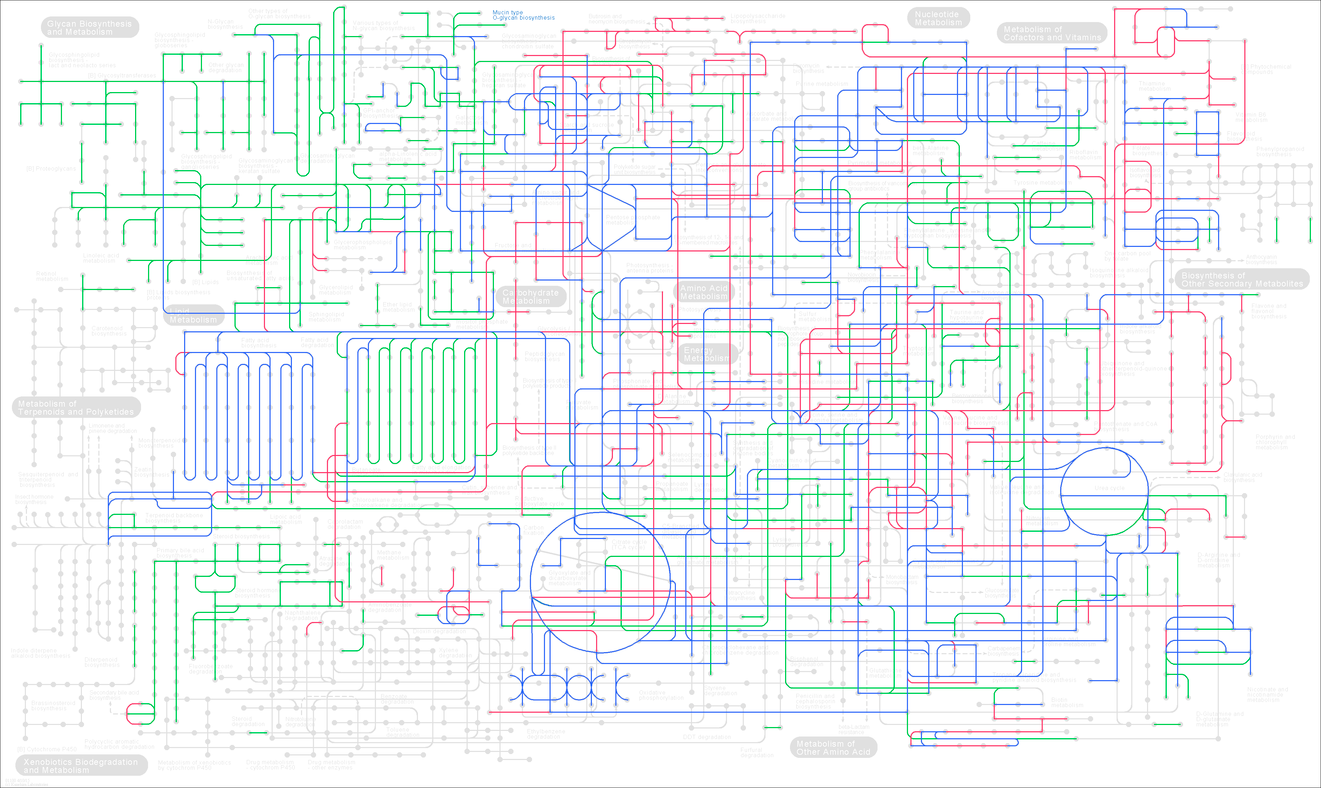
\includegraphics[scale=0.25]{human_metabolism_kegg.png}
%\end{frame}

%%%%%%%%%%%%%%%%%%%%%%%%%%%%%%%%%%%%%%%%%
\begin{frame}{Cast of characters}

\begin{itemize}
\item Simulation begins at time $0$ and proceeds in continuous time.
\item $\mathcal{R}_j$ is a chemical reaction.
\item $R_j(t) \in \mathbb{Z}_{\geq 0}$ counts occurrences of $\mathcal{R}_j$ up to time $t$.
\item $\theta_j\in \mathbb{R}_{\geq 0}$ is the rate at which $\mathcal{R}_j$ happens. More on this in future slides.
\item $X_i(t)  \in \mathbb{Z}_{\geq 0}$ is the number of molecules of type $i$
\item $\mathcal{D}_t \in \mathbb{R}$ is an incomplete observation of $X(t)$ with error.
\end{itemize}

\end{frame}
%%%%%%%%%%%%%%%%%%%%%%%%%%%%%%%%%%%%%%%%%
\begin{frame}{Wilkinson's eXample--reaction requirement}
\begin{figure}
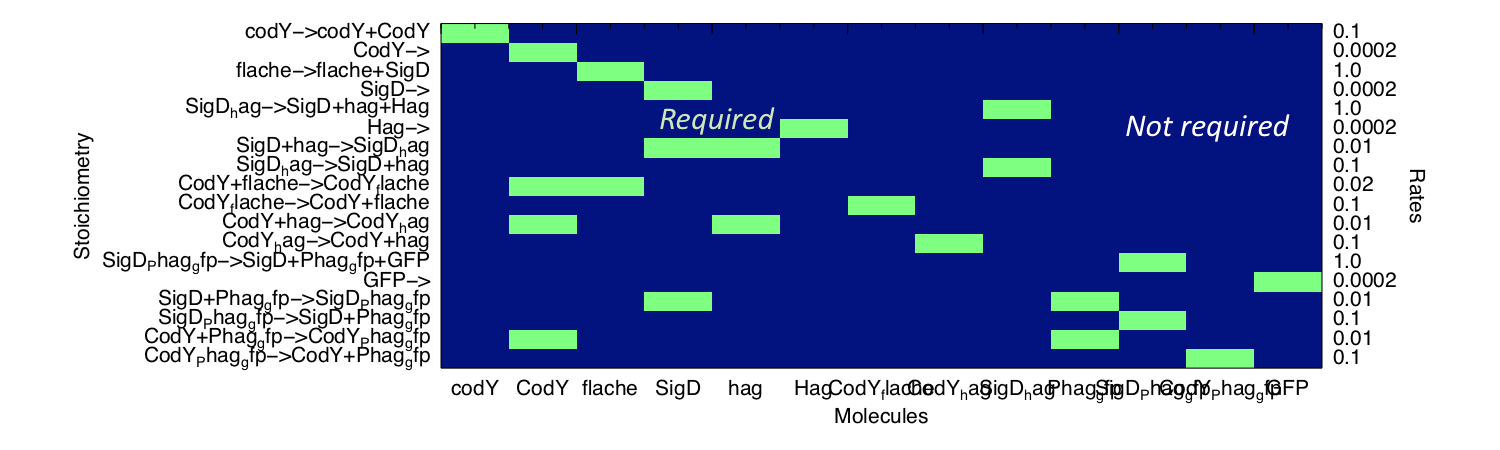
\includegraphics[scale=0.22]{rmat_fig.png}
\caption{\label{fig:entry} Roles of chemicals in various reactions. Green means the molecule is involved and blue means no involvement.}
\end{figure}
$$R_1(t)\sim PP(\theta_1 X_1(t))$$
$$R_5(t)\sim PP(\theta_5 X_4(t)X_5(t))$$
\end{frame}

%%%%%%%%%%%%%%%%%%%%%%%%%%%%%%%%%%%%%%%%%
\begin{frame}{Wilkinson's eXample--net change}
\begin{figure}
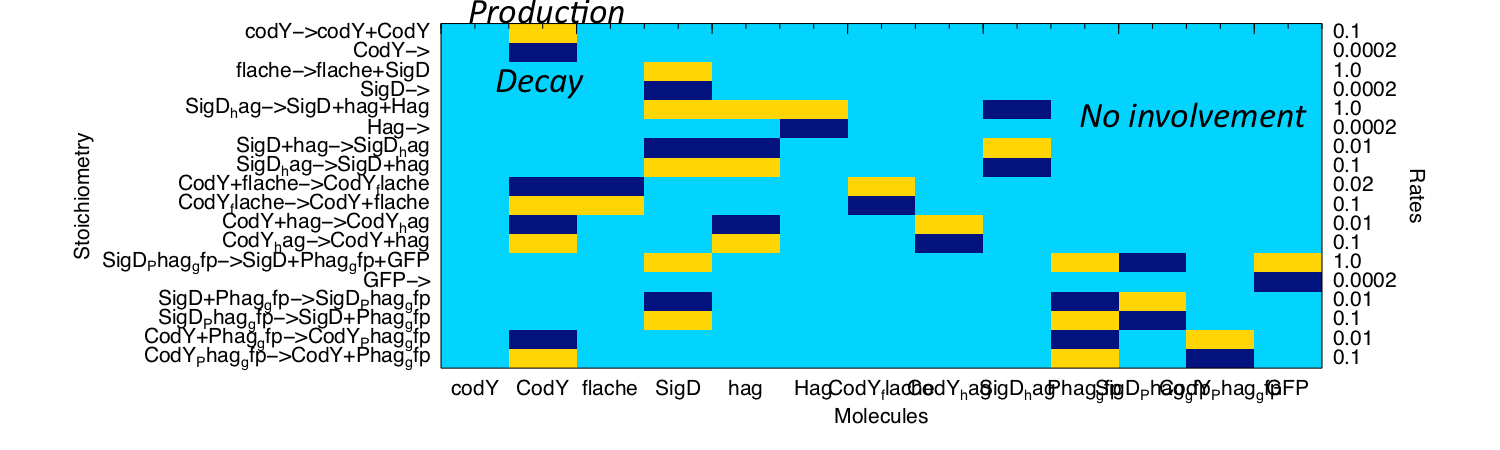
\includegraphics[scale=0.22]{sto_fig.png}
\caption{\label{fig:stoich} Roles of chemicals in various reactions. Green means the molecule is involved and blue means no involvement.}
\end{figure}
$$R_1(t)\sim PP(\theta_1 X_1(t))$$
$$R_5(t)\sim PP(\theta_5 X_4(t)X_5(t))$$
\end{frame}

%%%%%%%%%%%%%%%%%%%%%%%%%%%%%%%%%%%%%%%%%
\begin{frame}{Some notes}

\begin{itemize}
\item Assume reaction $\mathcal{R}_j$ occurs independently of the others (given the state).\item Priors on $\theta$ and $X(0)$, plus the dynamics already mentioned, determine the whole system.
\item EXact forward simulations are easy.
\end{itemize}
\end{frame}

%%%%%%%%%%%%%%%%%%%%%%%%%%%%%%%%%%%%%%%%%
\begin{frame}{Forward simulation}


\begin{algorithm}[H]
Given:\\
\Indp
Duration $T$ and initial particle counts $X(0)$\\
$S_{i,j}$, net change in molecules of type $i$ in a reaction of type $j$, and $P_{i,j}$ number of molecules of type $i$ entering a reaction of type $j$\\
$\theta$, a vector of reaction rates\\
\Indm
Do this:\\
\Indp
Initialize $X$ to $X(0)$ and $t$ to 0.\\
While true:\\
\Indp
Calculate $\alpha_j = \theta_j\prod_i {X_i\choose P_{ij}}$\\
Increment $t$ by EXponential(rate=$\sum_j \alpha_j$) \\
If $t > T$, quit and return $X$.\\
Otherwise, choose an integer $j$ with probability $\frac{\alpha_j}{\sum_j \alpha_j}$.\\
Increment $X$ by adding column $j$ of $S$.\\
\end{algorithm}


\end{frame}

%%%%%%%%%%%%%%%%%%%%%%%%%%%%%%%%%%%%%%%%%%
%\begin{frame}{Problem}
%\begin{figure}
%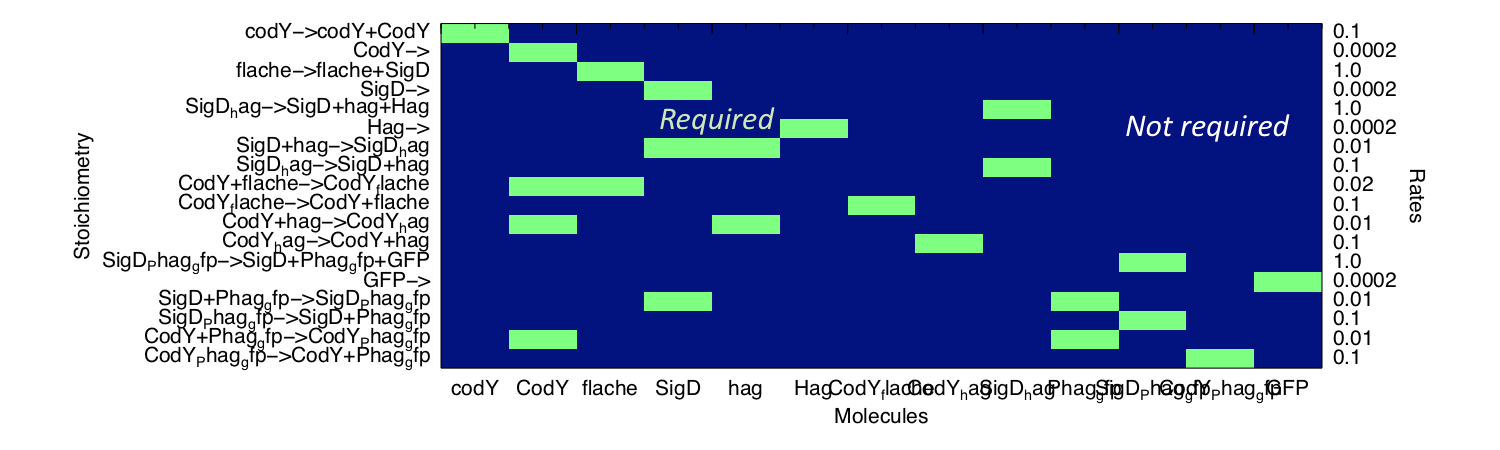
\includegraphics[scale=0.22]{rmat_fig.png}
%\caption{\label{fig:stoich} Roles of chemicals in various reactions. Green means the molecule is involved and blue means no involvement.}
%\end{figure}
%Given $\mathcal{D}_t$, find $\theta$. 
%\end{frame}

%%%%%%%%%%%%%%%%%%%%%%%%%%%%%%%%%%%%%%%%%
\begin{frame}{Likelihoods}
Likelihood if reaction $\nu_i$ happens at $t_i$: $$
\prod_{i=1}^\text{events} \theta_{\nu_{i}} \prod_{j=1}^\text{rXn types} {{X_{j}(t_{i-1})}\choose{p_{{\nu_{i}}j}}}\exp\left(-\theta_{\nu_{i}}
(t_i - t_{i-1}) {{X_j(t_{i-1})}\choose{p_{{\nu_{i}}j}}} \right)
$$

Likelihood from observing $X(t_i)$. Sum is over ``eligible'' paths for $\nu$ and integral is over a simpleX of possible wait-time tuples.
$$
\sum_{\nu}\int_{t} \prod_{i=1}^\text{events in $\nu$} \theta_{\nu_{i}} \prod_{j=1}^\text{rXn types} {{X_{j}(t_{i-1})}\choose{p_{{\nu_{i}}j}}}\exp\left(\text{same as above}\right).
$$

\end{frame}

%%%%%%%%%%%%%%%%%%%%%%%%%%%%%%%%%%%%%%%%%
\begin{frame}{Angles of attack}
Likelihood
$$
\sum_{\nu}\int_{t} \prod_{i=1}^\text{events in $\nu$} \theta_{\nu_{i}} \prod_{j=1}^\text{rXn types} {{X_{j}(t_{i-1})}\choose{p_{{\nu_{i}}j}}}\exp\left(-\theta_{\nu_{i}}
(t_i - t_{i-1}) {{X_j(t_{i-1})}\choose{p_{{\nu_{i}}j}}} \right).
$$

You might try:
\begin{itemize}
\item EM--still requires nasty sum.
\item Metropolis-Hastings on $\theta$--still requires likelihood evaluation.
\item Gibbs sampling--how do you update $\nu$?
\item Rejection sampling--most samples get rejected.
\end{itemize}

Solutions will need to either approXimate the likelihood or avoid it completely.

\end{frame}


%%%%%%%%%%%%%%%%%%%%%%%%%%%%%%%%%%%%%%%%%
\begin{frame}{A complication: measurement error}
If reactions occur at times $t_i$ and observations occur at times $s_k$, the likelihood becomes a sum over possible values of $X$ at times $s_0$, $s_1$, ... $s_\text{(num obs)}$ of:
\begin{align*}
& P(\mathcal{D}|X) \times \\
&\sum_{\nu}\int_{t} \prod_{i=1}^\text{events in $\nu$} \theta_{\nu_{i}} \prod_{j=1}^\text{rXn types} {{X_{j}(t_{i-1})}\choose{p_{{\nu_{i}}j}}}\exp\left(-\theta_{\nu_{i}}
(t_i - t_{i-1}) {{X_j(t_{i-1})}\choose{p_{{\nu_{i}}j}}} \right).
\end{align*}

%This raises a question: is it actually easier to sum out the possible reaction sequences/times  $\nu, t$ at the same time as the possibilties for $X(s_1)$, ... $X(s_\text{num obs})$?

\end{frame}
%%%%%%%%%%%%%%%%%%%%%%%%%%%%%%%%%%%%%%%%%
\begin{frame}{Another view of the problem}
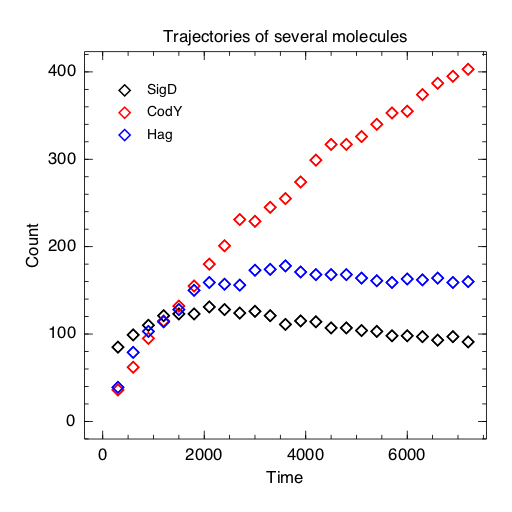
\includegraphics[scale=0.30]{simulated_data_multiple_mols.png}
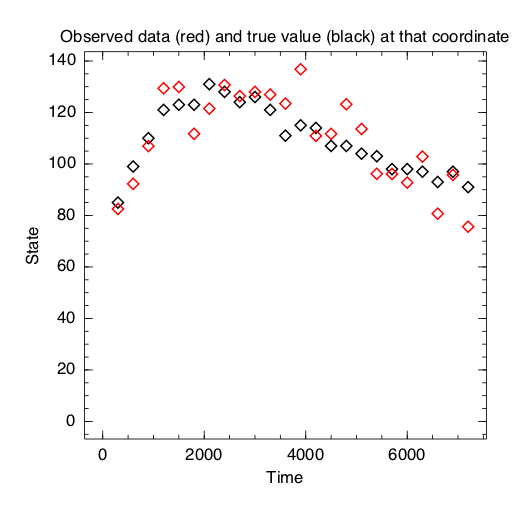
\includegraphics[scale=0.30]{simulated_data_obs.png}
\end{frame}

%%%%%%%%%%%%%%%%%%%%%%%%%%%%%%%%%%
%\begin{frame}{Other work}
%\begin{itemize} 
%\item Approximate MJP with SDE \cite{golightly2005bayesian,bayes_stoch_mod,fearnhead2014inference}
%
%\item Method of moments \cite{milner2013moment,zechner2012moment}
%
%\item Variational inference with mean-field approXimation  \cite{opper2008variational} 
%
%\item ApproXimate Bayesian Computation (ABC) and MCMC
%\cite{owen2014ABC_LF-MCMCcomparison,owen2014scalable,hobolth2009simulation,zechner2014scalable}
%
%
%\item EM with a sample average replacing the E-step expectation or similar \cite{gupta2014comparison,srivastava_rawlings2014stoch_opt,bayer2015stoch_em,horvath2008parameter,daigle2012accelerated}
%\end{itemize}


%\end{frame}
%%%%%%%%%%%%%%%%%%%%%%%%%%%%%%%%%%%%%%%%%
\begin{frame}{Likelihood free MCMC intro--the M-H recipe}

To produce a chain of samples from $P(\theta|D)$, using a proposal $q(\theta^*|\theta)$, accept with probability $p_{rej}(\theta^*|\theta)\equiv\min \{1, A\}$ if $$A=\frac{q(\theta,X|\theta^*,X^*)}{q(\theta^*,X^*|\theta,X)} \times \frac{P(\theta^*,X^*|\mathcal{D})}{P(\theta,X|\mathcal{D})}
$$

Can just as well use $\frac{P(\theta^*,X^*,\mathcal{D})}{P(\theta,X,\mathcal{D})}$.

\end{frame}
%%%%%%%%%%%%%%%%%%%%%%%%%%%%%%%%%%%%%%%%%
\begin{frame}{Likelihood Free MCMC}

\begin{align*}
&\frac{q(\theta^*, X^*|\theta, X)}{q(\theta, X|\theta^*, X^*)}
\times 
\red{\frac{P(X| \theta)}{P(X^*| \theta^*)}} 
\frac{ P( \theta)}{ P( \theta^*)} 
\frac{P(\mathcal{D}|X, \theta)}{P(\mathcal{D}|X^*, \theta^*)}\\
&=\frac{f(\theta^*|\theta)}{f(\theta|\theta^*)}
\red{\frac{P(X^*| \theta^*)}{P(X| \theta)} }
\times 
\red{\frac{P(X| \theta)}{P(X^*| \theta^*)} } 
\frac{ P( \theta)}{ P( \theta^*)}
\frac{P(\mathcal{D}|X, \theta)}{P(\mathcal{D}|X^*, \theta^*)}\\
&=\frac{f(\theta^*|\theta)}{f(\theta|\theta^*)}
\times 
\frac{ P( \theta)}{ P( \theta^*)} 
\frac{P(\mathcal{D}|X, \theta)}{P(\mathcal{D}|X^*, \theta^*)}.
\end{align*}
This approach, from 2003, is due to Marjoram et al. (paper title: ``MCMC Without Likelihoods'') \cite{Marjoram23122003}. 
\end{frame}

%%%%%%%%%%%%%%%%%%%%%%%%%%%%%%%%%%%%%%%%%
\begin{frame}{Wilkinson's adaptation of LF-MCMC}
LF-MCMC fails for the same reason as everything else: $P(\mathcal{D}|X, \theta)$ is tiny for almost all $X$ resulting from simulations.\\
\phantom{0}
The graphic on the following slides is from \cite{FinkeSMCslides}.
\end{frame}
\setbeamercolor{background canvas}{bg=}
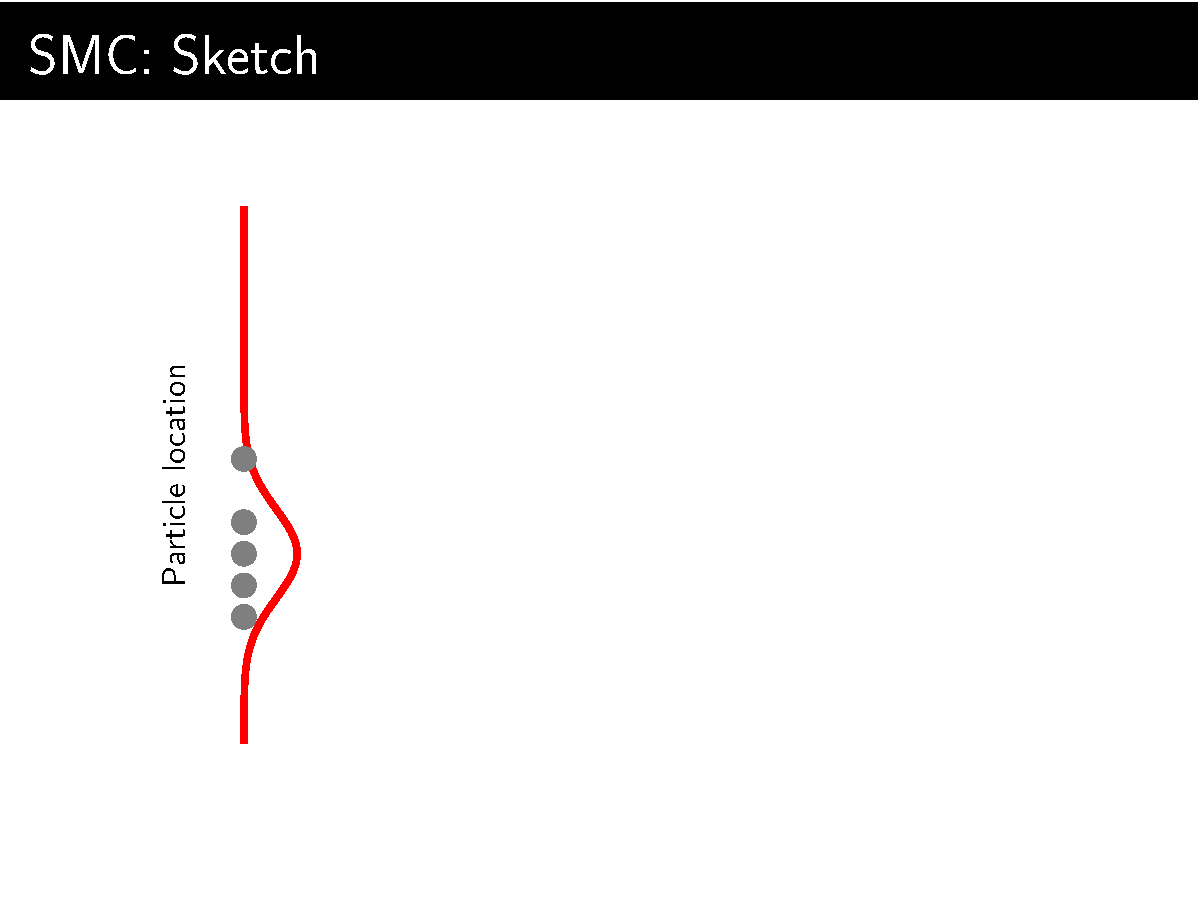
\includepdf[pages=-]{wonderful_smc_graphic_export}
%%%%%%%%%%%%%%%%%%%%%%%%%%%%%%%%%%%%%%%%%
%\begin{frame}{Likelihood Free Particle MCMC}
%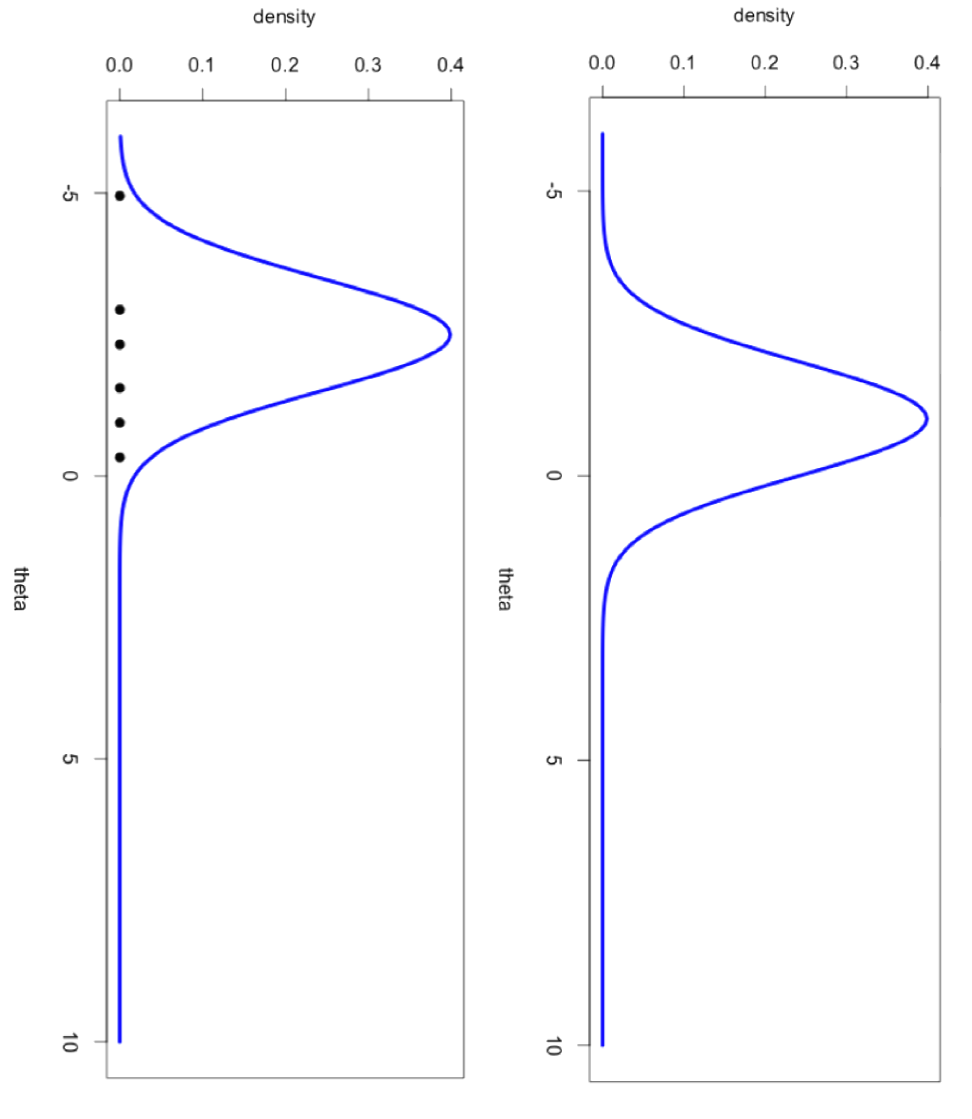
\includegraphics[scale=0.35]{prior_sample_graphic.png}
%\end{frame}
%\begin{frame}{Likelihood Free Particle MCMC}
%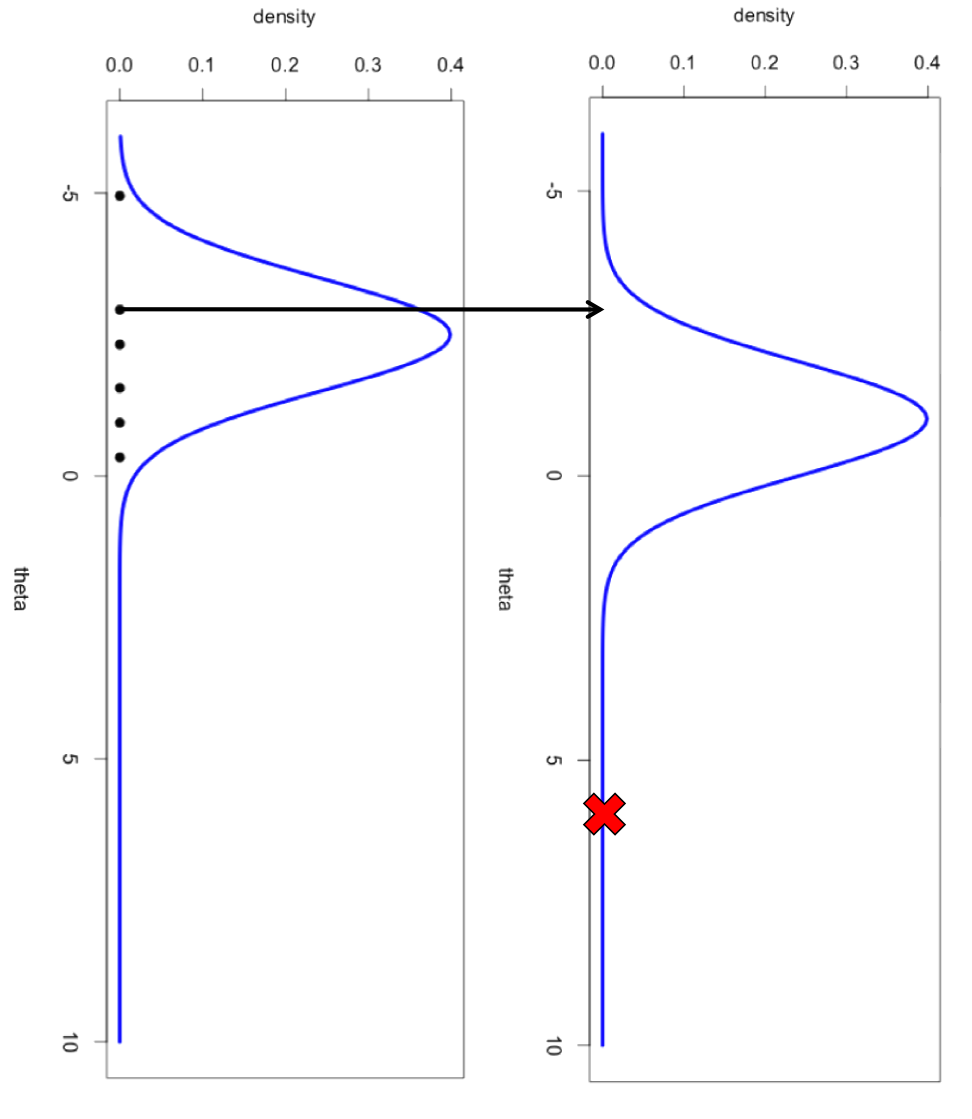
\includegraphics[scale=0.35]{post_sample1_graphic.png}
%\end{frame}
%\begin{frame}{Likelihood Free Particle MCMC}
%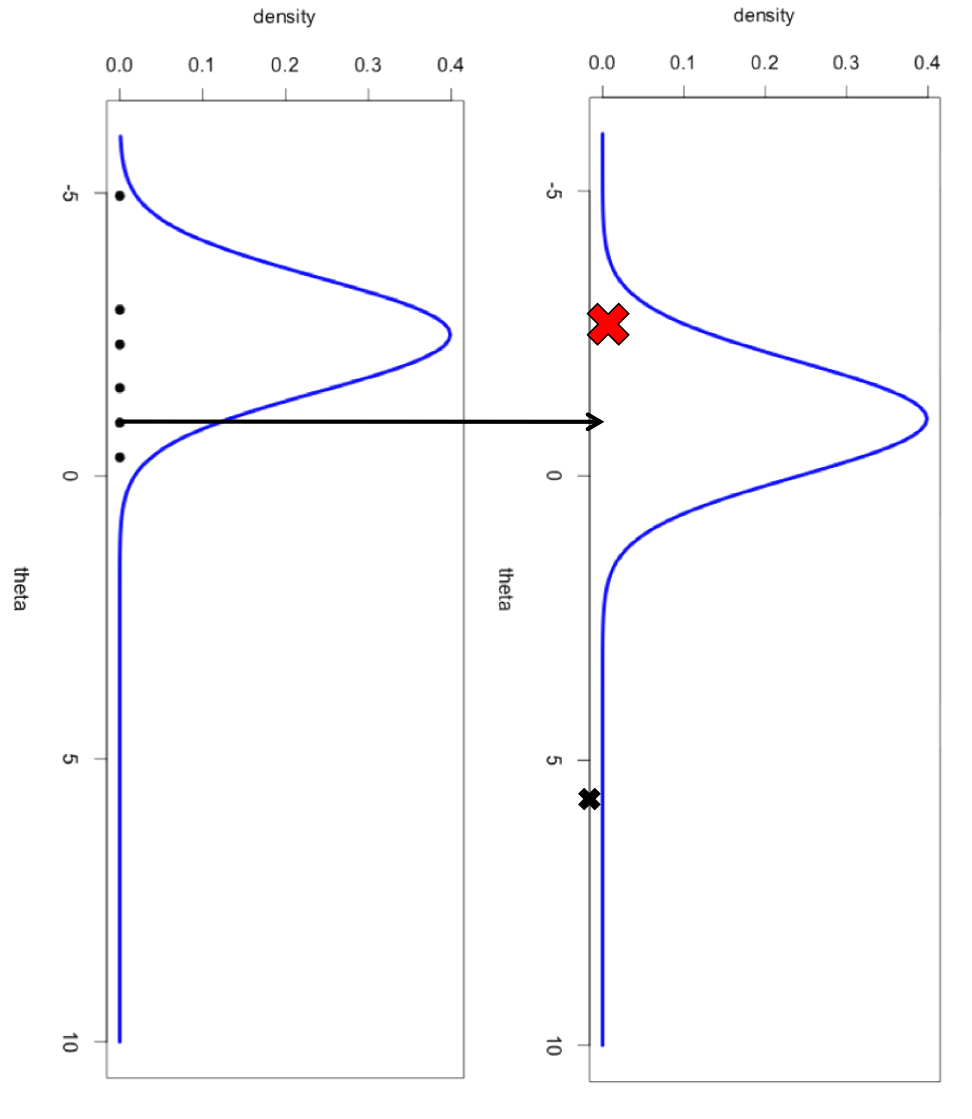
\includegraphics[scale=0.35]{post_sample2_graphic.png}
%\end{frame}
%\begin{frame}{Likelihood Free Particle MCMC}
%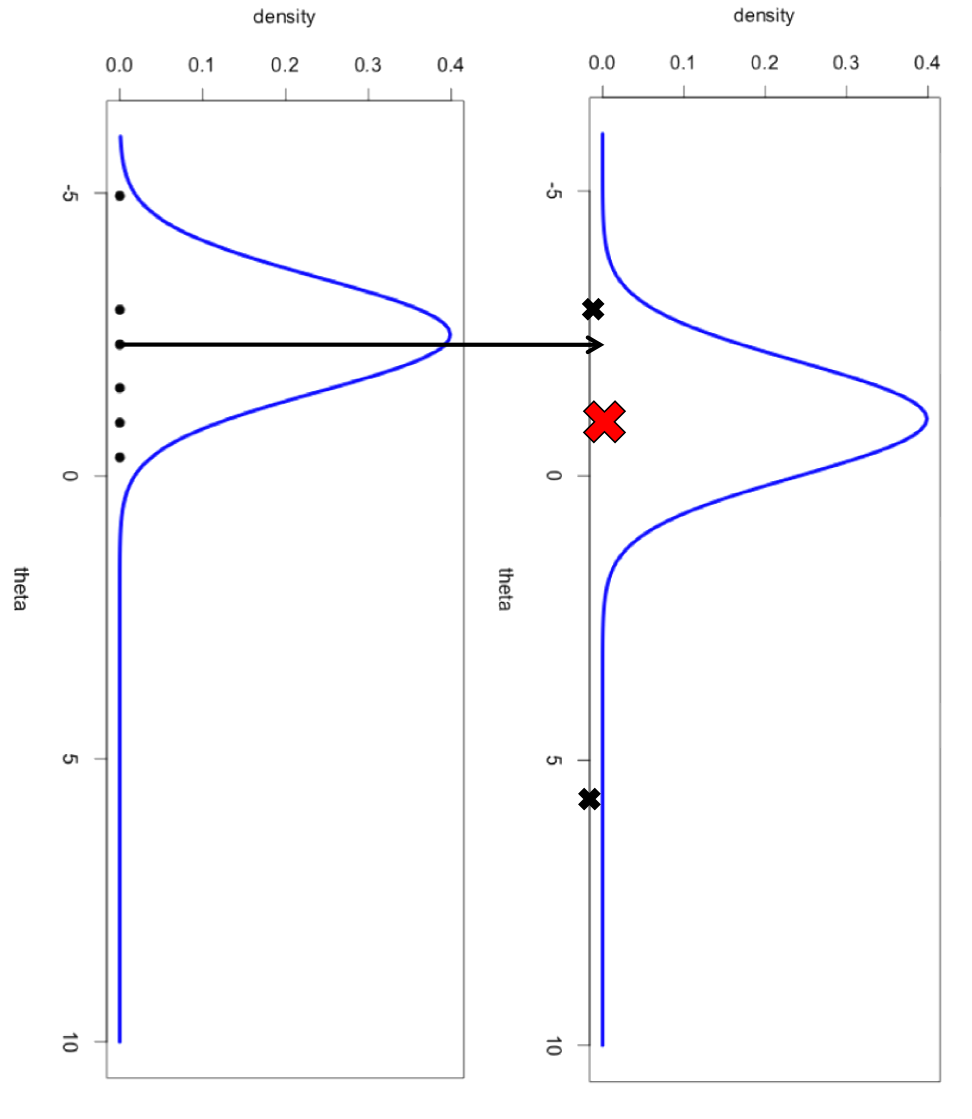
\includegraphics[scale=0.35]{post_sample3_graphic.png}
%\end{frame}
%\begin{frame}{Likelihood Free Particle MCMC}
%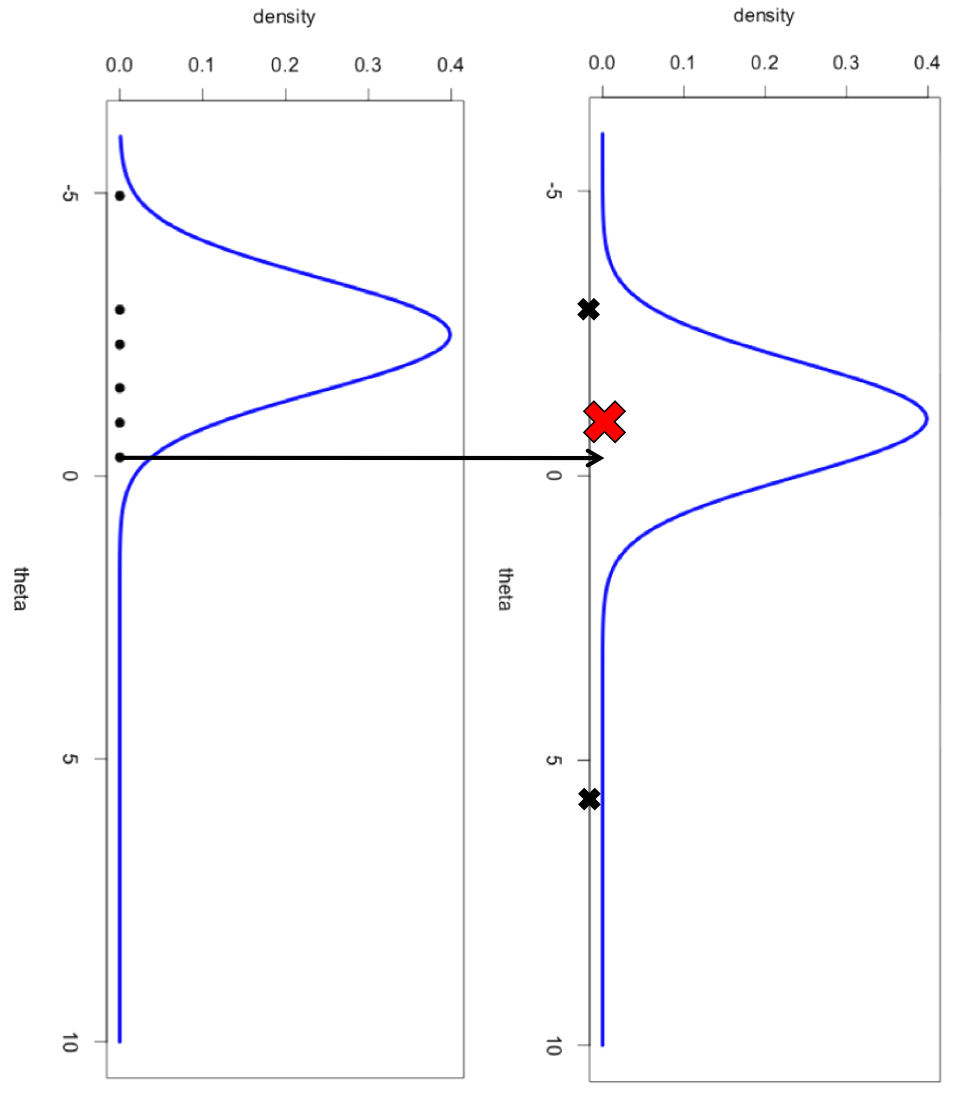
\includegraphics[scale=0.35]{post_sample4_graphic.png}
%\end{frame}
%\begin{frame}{Likelihood Free Particle MCMC}
%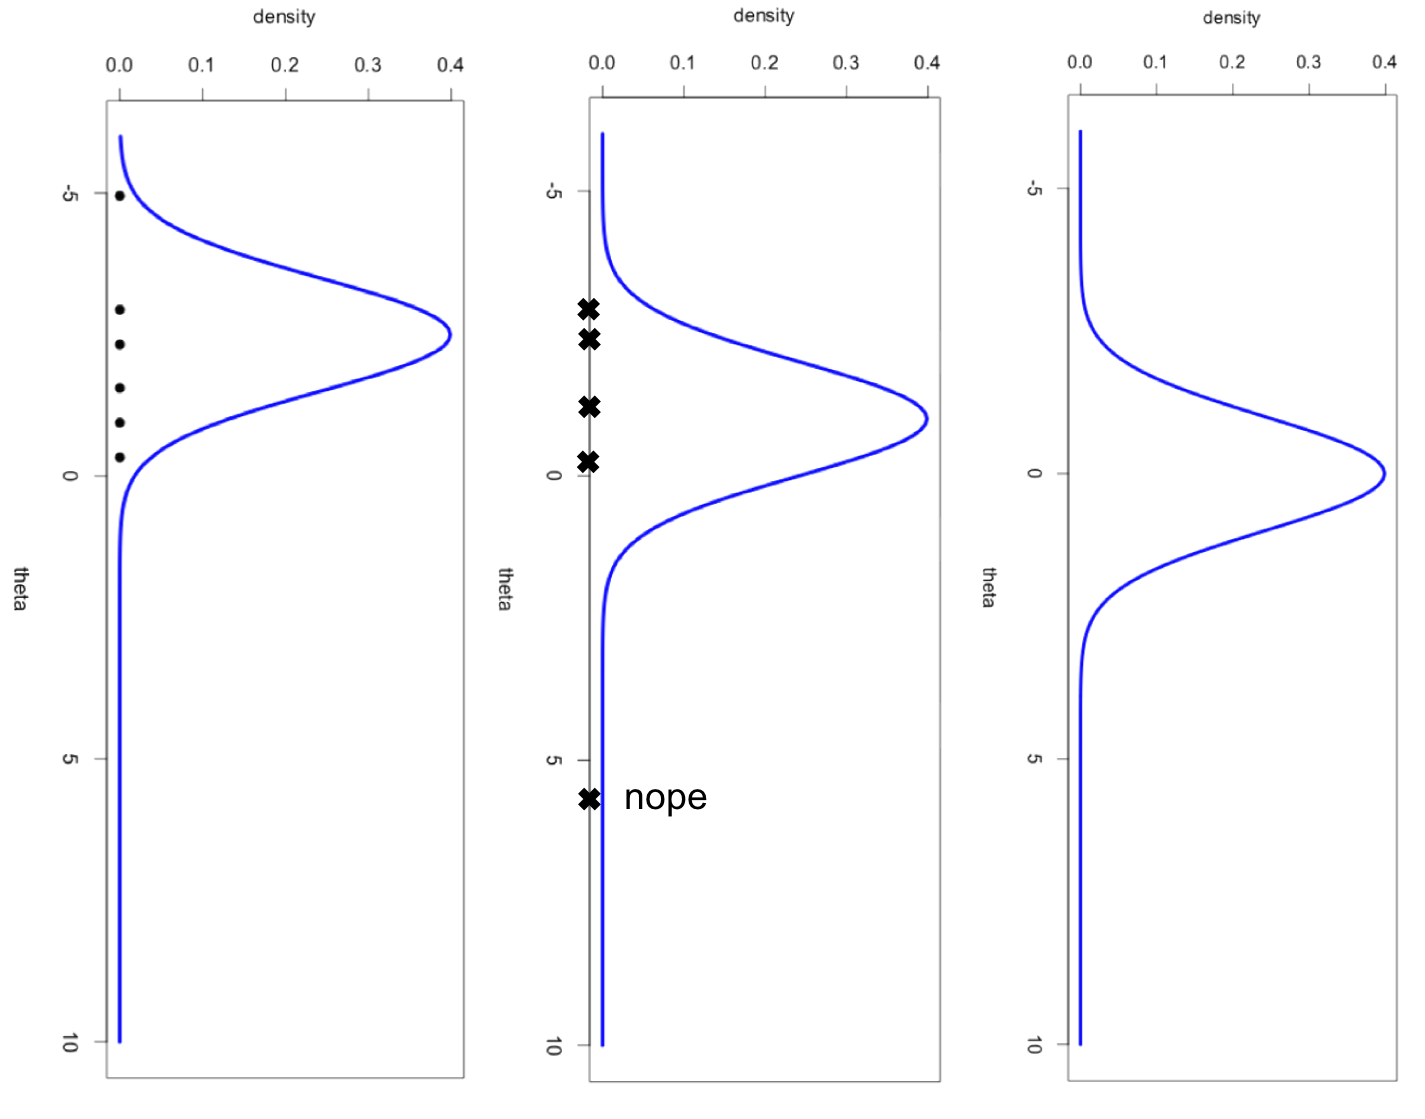
\includegraphics[scale=0.35]{post_sample5_graphic.png}
%\end{frame}
%\begin{frame}{Likelihood Free Particle MCMC}
%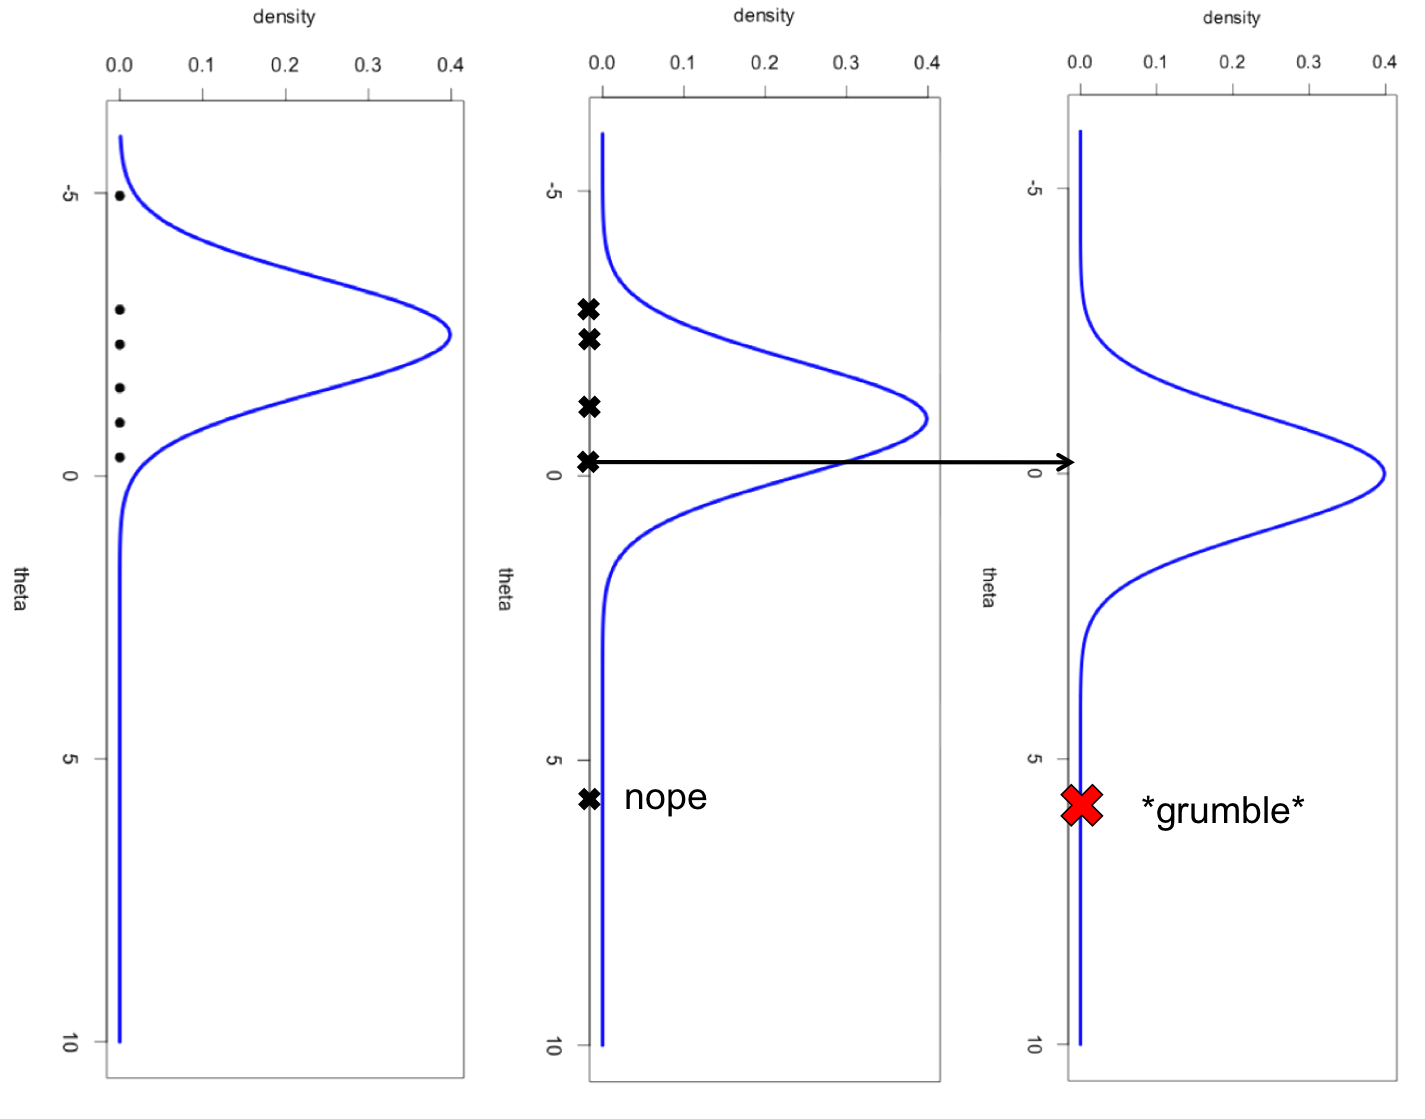
\includegraphics[scale=0.35]{post_sample6_graphic.png}
%\end{frame}

%%%%%%%%%%%%%%%%%%%%%%%%%%%%%%%%%%%%%%%%%%
\begin{frame}{Likelihood Free Particle MCMC}

\begin{algorithm}[H]
Given a hidden continuous-time Markov process $\{X_t\}_{t=0}^T$ with: \\
\Indp \Indp
Unknown parameters $\theta$ and known initial state $X_0$\\
Data points $\mathcal{D}_{t_{i}}$ at times $t_{i}$, $i \in \{1, ... I\}$ \\
A simple, tractable error model $P(\mathcal{D}_{t_{i}}|X_{t_{i}}, \theta)$\\
A simulator for paths of $X$ given $\theta$\\
An array $B_0$ of 1,000,000 samples from a prior on $\theta, X_0$\\
Empty arrays $B_{i}$ of the same length\\

\Indm \Indm
For each time point (for $i \in \{1, ... I\}$):\\
\Indp\Indp
Until $B_{i}$ is full: \\
\Indp\Indp
Draw $(\theta^*, X_{t_{i-1}}^*)$ from $B_{i-1}$ or a KDE of its contents\\
Using $(\theta^*, X_{t_{i-1}}^*)$, simulate up to $X_{t_{i}}^*$, the state at time $t_{i}$ \\
Set $A=\min(1, \frac{P(\mathcal{D}_{t_{i}}|X_{t_{i}}^*, \theta^*)}{P(\mathcal{D}_{t_{i}}|X_{t_{i}}, \theta)})$\\
With probability $A$, overwrite $(\theta, X_{t_{i}})$ with $(\theta^*, X_{t_{i}}^*)$\\
After burn-in and thinning, add $(\theta, X_{t_{i}})$ to $B_{i}$\\

\end{algorithm}
\end{frame}
%%%%%%%%%%%%%%%%%%%%%%%%%%%%%%%%%%%%%%%%%%
\begin{frame}{Likelihood Free Particle MCMC}

In place of the posterior, use this joint pdf: $P(\mathcal{D}_{t_{i}}, x(t_{1:i}), \theta|\mathcal{D}_{t_{i:i-1}}).$
\begin{align*}
&\overbrace{\frac{P(X(t_{1:i-1})^*,\theta^*| \mathcal{D}_{t_{1:i-1}})}{P(X(t_{1:i-1}), \theta| \mathcal{D}_{t_{1:i-1}})}}^{\text{induction hypothesis}}
%
\underbrace{\frac{P(X(t_{i})^*| X(t_{1:i-1})^*,\theta^*\gray{, \mathcal{D}_{t_{1:i-1}}})}{P(X(t_{i})| X(t_{1:i-1}), \theta \gray{, \mathcal{D}_{t_{1:i-1}}})}}_{\text{forward simulation}}
%
\times \\
%
&\overbrace{\frac{ P(X(t_{1:i-1}), \theta| \mathcal{D}_{t_{1:i-1}})}{ P( X(t_{1:i-1})^*,\theta^*| \mathcal{D}_{t_{1:i-1}})} }^{\text{For that joint PDF, start here...}}
%
\underbrace{\frac{P(X(t_{i})| X(t_{1:i-1}), \theta \gray{, \mathcal{D}_{t_{1:i-1}}})}{P(X(t_{i})^*| X(t_{1:i-1})^*,\theta^*\gray{, \mathcal{D}_{t_{1:i-1}}})}}_{\text{...then look here...}}\\
%  
&\underbrace{\frac{P(\mathcal{D}_{t_{i}}|X(t_{i}), \theta\gray{, \mathcal{D}_{t_{1:i-1}}})}{P(\mathcal{D}_{t_{i}}|X(t_{i})^*, \theta^*\gray{, \mathcal{D}_{t_{1:i-1}}})}}_{\text{...and finally, look here.}}
%
.\end{align*} 
\end{frame}

%%%%%%%%%%%%%%%%%%%%%%%%%%%%%%%%%%%%%%%%%
\begin{frame}{Does it mix?}
Bivariate marginals of the distribution of production (vertical) and decay (horizontal) log rates in a simple system. From left to right, distributions condition on zero data points, one, two, three, four, and 24.
\begin{center}
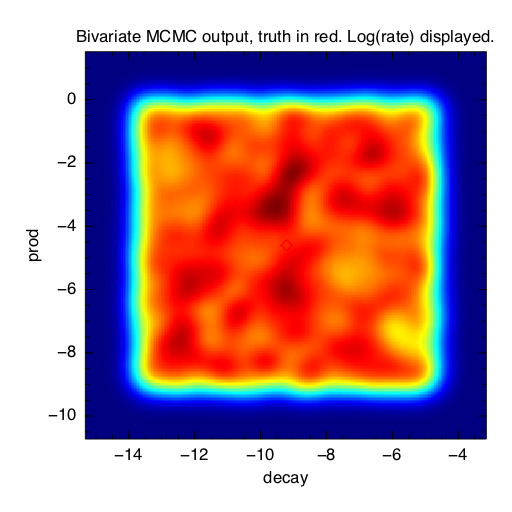
\includegraphics[height=1in,width=1in]{simple_million_stagewise_plots/dist0_contour_decay_prod.png}
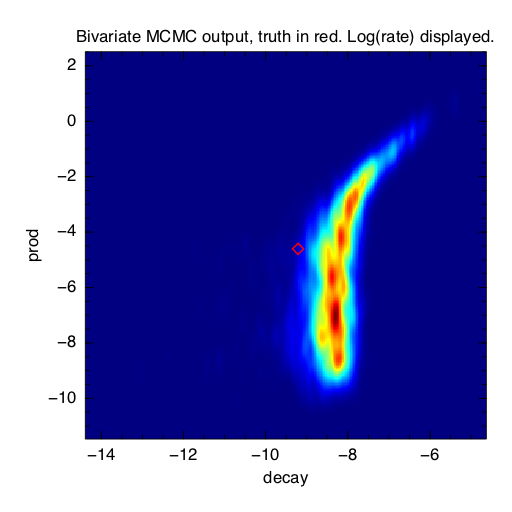
\includegraphics[height=1in,width=1in]{simple_million_stagewise_plots/dist1_contour_decay_prod.png}
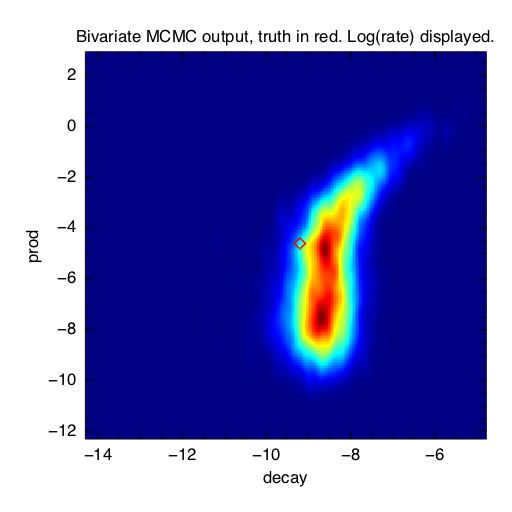
\includegraphics[height=1in,width=1in]{simple_million_stagewise_plots/dist2_contour_decay_prod.png}
\end{center}
\begin{center}
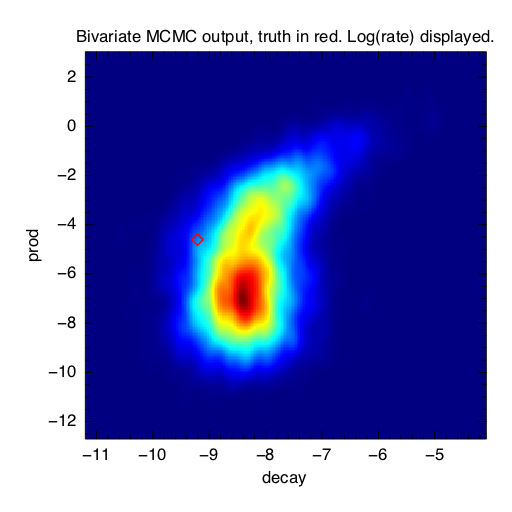
\includegraphics[height=1in,width=1in]{simple_million_stagewise_plots/dist3_contour_decay_prod.png}
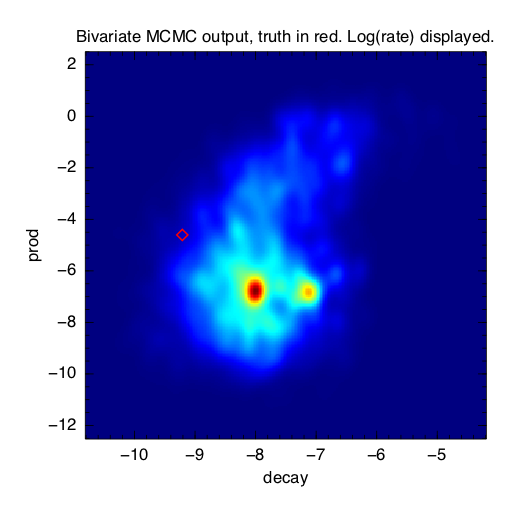
\includegraphics[height=1in,width=1in]{simple_million_stagewise_plots/dist4_contour_decay_prod.png}
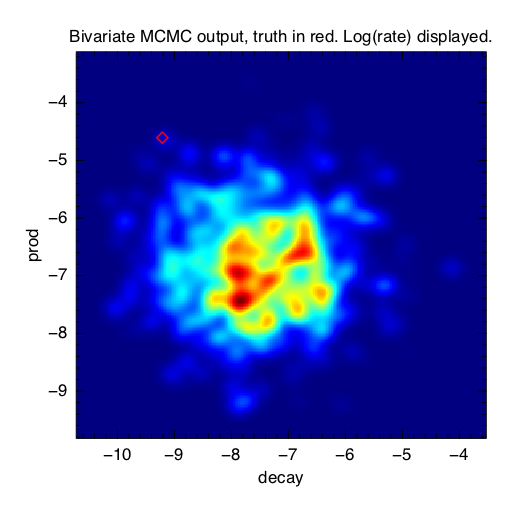
\includegraphics[height=1in,width=1in]{simple_million_stagewise_plots/dist23_contour_decay_prod.png}
\end{center}
\end{frame}
%%%%%%%%%%%%%%%%%%%%%%%%%%%%%%%%%%%%%%%%%
\begin{frame}{Sample Impoverishment}

\end{frame}
%%%%%%%%%%%%%%%%%%%%%%%%%%%%%%%%%%%%%%%%%

\begin{frame}[allowframebreaks]{Questions?}
\bibliographystyle{splncs}
\bibliography{prelim_biblio}
\begin{center}

 %\includegraphics[ trim={0cm 0cm 0 0},clip, width = .75\textwidth]{nice_things.jpeg}
\end{center}
\end{frame}
%%%%%%%%%%%%%%%%%%%%%%%%%%%%%%%%%%%

\end{document}